% Compile with XeLaTeX and the ACM acmart package, or select XeLaTeX in Overleaf.
\documentclass[sigconf,nonacm]{acmart}
\settopmatter{printacmref=false,printfolios=true,authorsperrow=3}
\setcopyright{none}
\title{Evaluating LLM-Selected Test Oracles for Underspecified Natural-Language Requirements}

\author{Ly The An}
\email{24520001@gm.uit.edu.vn}
\affiliation{\institution{VNUHCM - University of Information Technology}\city{Ho Chi Minh City}\country{Vietnam}}

\author{Luong Xuan Bao}
\email{24520161@gm.uit.edu.vn}
\affiliation{\institution{VNUHCM - University of Information Technology}\city{Ho Chi Minh City}\country{Vietnam}}

\author{Nguyen Do Gia Bao}
\email{24520165@gm.uit.edu.vn}
\affiliation{\institution{VNUHCM - University of Information Technology}\city{Ho Chi Minh City}\country{Vietnam}}

\author{Le Nguyen Thai Binh}
\email{24520194@gm.uit.edu.vn}
\affiliation{\institution{VNUHCM - University of Information Technology}\city{Ho Chi Minh City}\country{Vietnam}}

\author{Nguyen Thi Thanh Truc}
\email{trucntt@uit.edu.vn}
\affiliation{\institution{VNUHCM - University of Information Technology}\city{Ho Chi Minh City}\country{Vietnam}}


\usepackage{graphicx}
\usepackage{balance}
\emergencystretch=1em

\urlstyle{same}
\Urlmuskip=0mu plus 1mu\relax

\begin{document}
\begin{abstract}
Large language models can select expected test outcomes that natural-language requirements leave undecided. We evaluate requirement support, retention, and qualified fault detection when assertion selection is filtered by agreement with deterministic rules. The diagnostic pilots use 12 controlled threshold pairs and six FastAPI requirement pairs with 17 RESTestBench mutants. A matched API follow-up compares Qwen2.5-0.5B-Instruct and Qwen2.5-7B-Instruct and transfers the frozen rules to four held-out TodoApp pairs. On vague FastAPI requirements, filtered supported coverage rises from 18/48 at 0.5B to 20/48 at 7B, while qualified detections move from 22/51 to 21/51. The intersection retains 18/31 and 20/36 of the respective models' supported choices. On vague TodoApp requirements the rules select no status checks, leaving both models with 12/12 empty filtered suites. A larger model improves absolute retained coverage in parts of the sample. Rule coverage still limits what the intersection can retain.
\end{abstract}
\keywords{Requirements-Based Testing, Large Language Models, Test Oracles, Natural-Language Requirements, Mutation Testing, REST APIs}
\maketitle
\pagestyle{plain}\thispagestyle{plain}\raggedbottom
\section{Introduction}
Requirements-based test generation connects stakeholder intent to observable software behavior. A generated test needs an executable setup, an input or action sequence, and an oracle that decides whether its observed result is acceptable. Advances in language models make the translation from informal requirements to test artifacts increasingly practical, while the oracle problem continues to require careful treatment of expected behavior \cite{barr2015,yang2025,wang2024survey}.

A requirement can describe a valid objective while leaving its implementation choices open. Consider a requirement that another user's item must be inaccessible. It supports a rejection check under an agreed API interpretation. An assertion about one exact error code or message needs additional textual evidence. A generated assertion can agree with the current implementation and still impose a detail that the requirement leaves undecided. Conversely, a broad rejection check can follow the requirement and miss a fault that changes only an error message.

These distinctions matter when evaluating language-model-generated tests. A suite may execute successfully on a reference service yet include an unsupported assumption. A suite may contain only supported checks yet detect relatively few mutants. A filtering step can improve the first property while removing useful checks. Studying these outcomes together makes the practical effect of conservative filtering visible.

We examine this issue in a diagnostic pilot study with a deliberately constrained task. Inputs, API request sequences, and candidate assertion menus are fixed. A small local model selects expected outcomes. A deterministic rule selector separately examines the visible requirement. Their intersection produces a filtered suite. The contribution is to quantify the trade-off between requirement support and supported retention under a fixed candidate space, with nonemptiness and qualified fault detection assessed jointly. The empirical scope is the selection stage of LLM-based test case generation from natural-language requirements.

\textbf{RQ1} asks how many selected assertions lack support in the requirement. \textbf{RQ2} asks how many supported assertions survive filtering. \textbf{RQ3} asks how many seeded faults are detected by nonempty, supported suites that pass the reference implementation. \textbf{RQ4} asks how model size changes retention and qualified fault detection in the FastAPI pilot, and how frozen rules transfer to held-out TodoApp requirements. The controlled and API pilots address RQ1--RQ3. The paired API study addresses RQ4.

The controlled experiment contains 12 pairs of complete and incomplete threshold requirements, seven inputs per variant, two generation prompts, and three seeds, giving 144 model completions. The API experiment uses six precise/vague requirement pairs and 17 associated FastAPI mutants from RESTestBench \cite{kogler2026bench,restestrepo}. It contains 36 model completions and 23 recorded API observations. The API observations are shared when evaluating the three selection configurations.

The study contributes an assertion-level evaluation of requirement support, a comparison of model selection, text rules, and their intersection, and an auditable breakdown by requirement and seed. We then repeat the API experiment with a 7B model and measure rule transfer on requirements from a different service. The follow-up tests how much a larger model can recover under the original filter and how much the filter depends on the development texts.

\section{Background and Problem Formulation}
\subsection{Expected Behavior and Requirement Support}
An oracle evaluates a behavior produced by a test execution. Assertions can check status codes, response values, relations between created and retrieved resources, or the outcome of a subsequent operation. The oracle literature distinguishes several information sources, including specifications, contracts, existing implementations, and domain knowledge \cite{barr2015}. In this study, support is judged against the requirement variant that the selector actually receives.

Let $r$ be a requirement and $C_r$ its finite assertion menu. Let $G_r\subseteq C_r$ contain assertions judged to follow from $r$ under the study's interpretation policy. The annotation policy accepts direct statements and selected immediate behavioral consequences. For example, a general denial of access is represented by a client-error check. The policy makes this mapping explicit so that it can be challenged and revised. It also treats exact status and detail checks as requiring more specific wording.

The controlled experiment gives support a finite semantics. The input domain is the integers from 0 to 10, and outputs are labels A, B, and C. A partial requirement defines a set of permissible interpretations. A probe outcome is determined when every permissible interpretation yields the same label. The selector should abstain when multiple labels remain possible. Thus, partial information can support some outcomes even when other outcomes for the same requirement remain undecided.

\subsection{Compatibility and Fault Detection}
Compatibility records whether a selected suite passes on the original service. Fault detection records whether a selected assertion fails on an associated mutant. The distinction between execution validity and behavioral adequacy also appears in recent requirement-to-test benchmarks and agent evaluations \cite{kogler2026bench,qi2026,shi2026}. We additionally require the suite's selected assertions to belong to $G_r$ before crediting a qualified mutant detection.

A mutant is an intentionally modified program version. Mutation testing can expose weaknesses in tests by changing observable behavior in controlled ways \cite{papadakis2019}. Property-based mutation testing ties the interpretation of a killed mutant to the property being tested \cite{bartocci2023}. We use the benchmark's requirement-associated mutants and separately report which ones are distinguishable by the available supported candidates.

\section{Related Work and Literature Search}
\subsection{Search Scope}
The literature search was updated on 19 November 2026. We used web-indexed scholarly searches with title verification through author repositories, arXiv, publisher pages, official model documentation, and research artifact repositories. Query families combined natural-language requirements with test generation, acceptance testing, assertion generation, test oracles, underspecification, ambiguity, grounding, and mutation testing. Searches also used the titles of the closest studies to identify related work and artifacts.

We retained sources relevant to requirement-driven generation, semantic oracle evaluation, fault detection, or the pilot implementation. The bibliography contains 28 scholarly publications or manuscripts and six technical or research-artifact sources. The targeted narrative synthesis is bounded by the queries, accessible records, and the search date. The source register records publication types, links, and roles. A survey artifact lists 267 primary RBTG studies for further screening \cite{rbtgdata}.

\subsection{From Requirements to Test Artifacts}
Requirements-based testing has a substantial history across requirement representations and generation methods \cite{yang2025}. A recent survey of AI-driven generation identifies ambiguity, traceability, and hallucination control as continuing concerns \cite{folorunsho2026}. UMTG derives executable acceptance tests from natural-language use cases and a domain model, using NLP and formal constraints \cite{wang2022umtg}. CiRA extracts conditionals from informal requirements and converts their relationships into acceptance tests \cite{fischbach2023}. These approaches motivate explicit links between a requirement's conditions and the checks a test performs.

RAGTAG uses retrieval-augmented language models to generate industrial test scenarios from requirements \cite{arora2024}. Ferreira et al. study a workflow from user stories to Gherkin scenarios and then Cypress scripts \cite{ferreira2025}. Masuda et al. generate high-level test cases using prompts and evaluate correspondence to existing tests \cite{masuda2025}. These settings emphasize useful scenarios and executable artifacts. Our pilots hold scenario construction fixed and examine the support of the assertions selected for those scenarios.

Several approaches enrich the generation process. Moradi et al. investigate LoRA-based adaptation for requirement-based test generation \cite{moradi2026}. RAFT integrates domain knowledge and formalized artifacts into compliance-test generation \cite{xue2026}. Cunha and Macedo study LLM-generated tests for validating Alloy specifications \cite{cunha2026}. These works suggest possible extensions involving model adaptation and explicit formal representations. The current experiment evaluates a fixed local model and a lightweight selector under a small, inspectable candidate space.

\subsection{Oracle Generation and Evaluation}
TOGA learns exceptional and assertion oracles from focal-method context \cite{dinella2022}. An extended evaluation by Hossain et al. investigates the reliability and fault-detection implications of neural oracle generation \cite{hossain2023}. Konstantinou et al. examine whether generated oracles capture actual program behavior or expected behavior \cite{konstantinou2024}. These studies motivate checking both what an oracle asserts and whether that assertion is a justified behavioral expectation.

Endres et al. evaluate natural-language-to-postcondition translation using correctness and discriminative power \cite{endres2024}. Molinelli et al. investigate test oracle generation using artifacts created after model training cutoffs \cite{molinelli2025}. Their evaluation highlights the importance of benchmark provenance. Ou\'edraogo et al. compare prompting strategies and models for unit test generation across correctness, readability, coverage, and bug detection \cite{ouedraogo2024}. Our fixed assertion-selection task enables direct analysis of each retained assertion.

Ma and Eisty generate Java oracle code from business requirements derived from real Defects4J bugs, evaluating agreement with a requirement-derived oracle and the fixed system \cite{ma2026}. Their setting is particularly close in its focus on requirement-driven oracles. Our setting pairs levels of requirement detail, constrains the output to a candidate menu, and measures how an intersection filter changes unsupported selections and supported retention. These design differences define the scope of the comparison.

\subsection{REST APIs and the Closest Benchmarks}
REST API testing must handle interface descriptions, authentication, state, and operation dependencies \cite{golmohammadi2024}. RESTest generates black-box tests from OpenAPI descriptions \cite{martinlopez2021}. RESTifAI constructs reusable API tests through a happy-path workflow and derived negative cases \cite{kogler2025restifai}. These methods provide context for the setup and execution problems that our frozen request sequences intentionally control.

RESTestBench supplies precise/vague requirements, API services, and requirement-associated mutants \cite{kogler2026bench}. ReqTestAgent connects ambiguity processing, test generation, and execution-based verification \cite{shi2026}. Req2Test-Bench evaluates repository-level requirement-to-test implementations and distinguishes passing tests from kill-complete behavior \cite{qi2026}. Our contribution is a local assertion-level analysis of the support/retention trade-off inside a fixed test context. The empirical comparisons in this paper are between the configurations actually run in our pilots. The discussion of external systems describes differences in tasks and evidence.

\section{Assertion Selection and Filtering}
\subsection{Three Selection Configurations}
Let $L(r)$ be the assertions selected by the language model and $R(r)$ those selected by the deterministic rules. The filtered selection is
\begin{equation}
F(r)=L(r)\cap R(r).
\end{equation}
The API pilot evaluates $L$, $R$, and $F$ on the same assertion menu, request sequence, and recorded API outcomes. The filter uses agreement between the model and the text rules. The semantic annotation set $G_r$ is used by the evaluator and is excluded from the generation prompt.

The intersection imposes a direct upper bound on retention. An assertion omitted by either selector is absent from $F$. If the rule set under-selects a supported assertion, the filter can discard a correct model choice. If a rule admits an unsupported assertion and the model also selects it, agreement alone would retain that assertion. This makes the observed reliability of the rule set part of the interpretation of the filter's results.

\begin{figure}[t]
\centering
\fbox{\parbox{0.90\columnwidth}{\centering Visible requirement, interface context,\\fixed actions, assertion menu}}
\par\smallskip $\downarrow$\par\smallskip
\begin{tabular}{cc}
\fbox{LLM selection $L$} & \fbox{Text-rule selection $R$}\\[5pt]
\multicolumn{2}{c}{$\downarrow$}\\[3pt]
\multicolumn{2}{c}{\fbox{Retain $F=L\cap R$}}
\end{tabular}
\par\smallskip $\downarrow$\par\smallskip
\fbox{Support, original pass, mutant checks}
\caption{Selection and evaluation in the API pilot. The evaluator applies a separate support annotation and shared execution observations to each configuration.}
\label{fig:selection}
\Description{The visible requirement and fixed test context feed an LLM selector and text-rule selector. Their intersection is evaluated for support, compatibility with the original service, and mutant detection.}
\end{figure}

\subsection{Model Inputs and Decoding}
The model is Qwen2.5-0.5B-Instruct in the Q4\_K\_M GGUF format \cite{qwen2024}, run locally using llama.cpp release b5046 \cite{llamacpp}. Saved generation settings use temperature 0.3, top-$k$ 40, top-$p$ 0.95, and seeds 11, 23, and 47. A seed initializes the sampling procedure. These three values define repeated draws under the same configuration.

In the controlled experiment, the model returns seven labels, each A, B, C, or an abstention symbol. The direct prompt requests a best guess when information is missing. The abstention prompt requests a label only when it follows from the requirement. The decoding grammar enforces the output alphabet and sequence length. It guarantees a parseable format while leaving the semantic choices to the model.

In the API experiment, each prompt contains a requirement variant, a fixed action sequence, an assertion menu, and a compact OpenAPI operation description. OpenAPI describes the API interface \cite{openapi}. The prompt explicitly asks for Y/N decisions and warns against using a general schema response to infer an exact error for a particular scenario. The model can omit an assertion by returning N. This is the operational meaning of abstention in the API pilot.

\subsection{Text Rules and Support Labels}
For threshold requirements, the rule selector parses controlled-language patterns and enumerates permissible comparators, cutoffs, and fallback labels. It retains a probe label when all admissible interpretations agree. The evaluator separately constructs expected labels from the saved scenario references. Both procedures embody the same finite semantics, making the rule-only baseline strong in this restricted setting.

For API requirements, rules match explicit status codes, field-equality descriptions, exact error-detail wording, and selected general success or rejection cues. The patterns were written after inspecting the sampled requirements. Some supported implications have no corresponding matched phrase, so rule coverage can be incomplete. The support labels were prepared as one study-authored annotation set. Agreement with the original service is checked for internal consistency. Independent annotation agreement remains a follow-up requirement for broader validation.

\section{Experimental Design and Data Provenance}
\subsection{Controlled Threshold Pilot}
The controlled dataset was constructed for this pilot. It contains 12 pairs of English requirements with one complete variant and one incomplete variant. Four pairs omit whether a boundary includes equality, four omit a bounded cutoff value, and four omit a fallback output label. Each variant is evaluated at inputs 0, 3, 4, 5, 6, 7, and 10. Service names are scenario labels for the same finite task.

For every requirement variant, both direct and abstention prompts run with three seeds. The number of actual model calls is therefore $12\times2\times2\times3=144$. Each call provides seven probe decisions. The filtered configuration reuses the abstention response and applies the text rules. The rules run deterministically once per requirement variant.

Across the incomplete requirements, 42 of the 84 probe positions have a unique supported output and 42 remain underdetermined. Repetition across three seeds creates 126 supported and 126 underdetermined probe opportunities for each model-based configuration. These are repeated positions on the same 12 requirements. They define the counting unit used in the controlled results.

\subsection{RESTestBench FastAPI Pilot}
The API dataset is a purposive sample from RESTestBench, fixed at repository commit \texttt{4decc1e}. The companion audit records the full commit identifier. The selected requirement identifiers are 2, 3, 4, 6, 13, and 34. Each has a precise and a vague version. We use the corresponding FastAPI service, which is based on the Full Stack FastAPI Template \cite{fastapi}. Table~\ref{tab:sample} shows the sampled tasks and their candidate and mutant counts.

\begin{table}[t]
\caption{Frozen API sample. $|G_p|$ and $|G_v|$ count supported candidates for precise and vague requirements in one deterministic pass.}
\label{tab:sample}
\centering\small
\begin{tabular}{r l r r r r}
\toprule
ID & Scenario & $|C|$ & $|G_p|$ & $|G_v|$ & Mut.\\
\midrule
2 & Retrieve created item & 8 & 6 & 5 & 3\\
3 & Retrieve missing item & 6 & 3 & 2 & 2\\
4 & Read another user's item & 7 & 3 & 1 & 3\\
6 & Update an owned item & 8 & 6 & 5 & 3\\
13 & Wrong-password login & 7 & 4 & 2 & 3\\
34 & Register new user & 8 & 5 & 1 & 3\\
\midrule
 & Total & 44 & 27 & 16 & 17\\
\bottomrule
\end{tabular}
\end{table}

The API generation count is $6\times2\times3=36$ completions. Every completion selects from six to eight candidate assertions. The 44 candidates summed across scenarios give 132 candidate decisions per requirement variant over the three seeds. Candidate menus deliberately contain both supported and unsupported choices.

Execution records contain six original scenario observations and 17 mutant observations. Each observation records the outcomes of the scenario's candidate checks. We then apply the raw and filtered selections to the same recorded outcomes. Consequently, 51 mutant opportunities per LLM configuration represent $17\times3$ scored evaluations. The underlying executions comprise 17 distinct mutant observations. Sharing these observations isolates assertion selection and avoids differences in service state across selectors.

\subsection{Evidence Files and Scoring}
The controlled archive contains requirement definitions, reference descriptions, the scoring program, and 144 saved generation records. The API archive contains requirement extracts, scenario definitions, the rule implementation, support labels, 36 saved model responses, 23 API observations, and detailed scoring tables. Raw model output is in \texttt{runs.jsonl}. The file \texttt{observations.jsonl} stores API outcomes. The labels appear in \texttt{semantic\_gold.json}. Per-case counts are in \texttt{comparison.csv}. Aggregates are in \texttt{summary.csv}.

For this expanded manuscript, the stored raw records were rescored and the aggregate tables were checked against the two-page paper. Per-requirement and per-seed results were derived from the same records. The additional breakdowns are secondary analyses of the existing pilot runs. Literature results are attributed to their respective sources and are used to position the study.

\subsection{Measures and Counting Units}
\label{sec:measures}
For a selector $S$ and support set $G_r$, we count $|S\cap G_r|$ supported selections and $|S\setminus G_r|$ unsupported selections. Supported coverage divides supported selections by available supported candidates. Unsupported proportion divides unsupported selections by all selected assertions. Both aggregate numerators and denominators are summed over the relevant scenarios and seeds.

A suite is qualified when it is nonempty, every selected assertion is supported, and every assertion passes on the original observation. Write this predicate as $Q(S,r)$. A mutant contributes one qualified detection when $Q(S,r)$ holds and at least one selected assertion fails on that mutant. The same suite can detect several mutants, while each mutant contributes at most once per scenario/seed evaluation.

The primary detection denominator is every associated mutant opportunity. A secondary denominator includes only mutants distinguishable by at least one candidate in $G_r$. For the vague variant, this is 13 of the 17 mutants, giving 39 observable opportunities across three seeds. Reporting both denominators exposes the candidate-space limit on fault detection.

\section{Results}
\subsection{RQ1: Unsupported Assertions}
Table~\ref{tab:threshold} reports the incomplete threshold requirements. The direct prompt supplied a label on 62 of 126 underdetermined opportunities. The abstention prompt reduced this count to 58. Applying the filter reduced the observed count to zero. The abstention prompt also returned an incorrect label on 34 determined opportunities. The filtered output contained no incorrect determined labels under the finite support semantics.

\begin{table}[t]
\caption{Incomplete threshold requirements. Supported retention uses determined probes. Unsupported output uses underdetermined probes. Model-based configurations include three seeds.}
\label{tab:threshold}
\centering\small
\begin{tabular}{l r r r}
\toprule
Method & Supported & Wrong on & Output on\\
 & retained & determined & underdetermined\\
\midrule
Direct & 30/126 & 45/126 & 62/126\\
Abstention & 29/126 & 34/126 & 58/126\\
Filtered & 29/126 & 0/126 & 0/126\\
Rules & 42/42 & 0/42 & 0/42\\
\bottomrule
\end{tabular}
\end{table}

For the API pilot, Table~\ref{tab:api} reproduces the six aggregate rows of the original manuscript. On precise requirements the raw model selected 73 assertions, of which 47 were supported and 26 unsupported. Filtering removed those 26 unsupported assertions. On vague requirements it selected 84 assertions, with 28 supported and 56 unsupported. The filter retained 17 assertions, all supported by the annotation set.

\begin{table*}[t]
\caption{Oracle selection and qualified fault detection on FastAPI. Supported is selected/available. Unsupported is unsupported/all selected. Original pass and qualified suites count nonempty suites. Each model-based row has 18 suites and 51 mutant opportunities. Rules have six suites and 17 mutant opportunities.}
\label{tab:api}
\centering
\begin{tabular}{llrrrrrr}
\toprule
Requirement & Method & Supported & Unsupported & Empty & Original pass & Qualified suites & Qualified kills\\
\midrule
Precise & LLM & 47/81 & 26/73 & 2/18 & 2/18 & 2/18 & 2/51\\
Precise & Filtered & 47/81 & 0/47 & 3/18 & 15/18 & 15/18 & 32/51\\
Precise & Rules & 27/27 & 0/27 & 0/6 & 6/6 & 6/6 & 17/17\\
\midrule
Vague & LLM & 28/48 & 56/84 & 0/18 & 2/18 & 0/18 & 0/51\\
Vague & Filtered & 17/48 & 0/17 & 6/18 & 12/18 & 12/18 & 19/51\\
Vague & Rules & 9/16 & 0/9 & 0/6 & 6/6 & 6/6 & 10/17\\
\bottomrule
\end{tabular}
\end{table*}

The unsupported proportion for vague raw selections is $56/84=66.7\%$. The filtered result is $0/17$. A smaller unsupported proportion describes better observed support among the assertions that remain. Empty suites are reported alongside it because an empty output contains no unsupported selections and provides no test oracle.

The zero counts depend on the rules and support policy used in these pilots. In the controlled language, enumeration directly implements the permissible interpretations. In the API sample, the patterns were tuned after inspection and happened to select only supported candidates. The observed result therefore establishes a property of these finite selections and annotations. An unseen phrase or a changed annotation policy could alter the outcome.

\subsection{RQ2: Supported Assertions Retained}
The controlled filter retained 29 of 126 determined probe outcomes, or 23.0\%. This is the same count of correct determined outcomes already supplied by the abstention prompt. Filtering removes the prompt's unsupported or incorrect choices while leaving those 29 correct ones. The rule-only selector provides all 42 determined outputs in its single pass.

The denominators reflect repetition. The 42 determined positions are counted three times for model-based configurations, giving 126. The rule selector runs once and has denominator 42. Its deterministic 100\% retention is consistent with its use of the controlled grammar and complete finite enumeration.

On vague API requirements, supported coverage falls from $28/48=58.3\%$ to $17/48=35.4\%$. The filter discards 11 previously selected supported assertions, or $11/28=39.3\%$ of the supported raw selections. It retains $17/28=60.7\%$ of them. The rule selector contains nine of 16 supported candidates in one pass, giving 56.3\% supported coverage.

On precise API requirements, all 47 supported raw selections survive. Coverage remains $47/81=58.0\%$. Available supported candidates total 27 per seed and 81 over three seeds. Preserving those 47 selections shows that the filter's retention cost varies with the text and the rule matches. It still leaves 34 supported opportunities unselected because the original model did not choose them.

Figure~\ref{fig:rates} shows the API support and detection rates together. The intersection has higher observed selection precision than the raw model, while the coverage measure exposes what was lost. Both measures are needed to interpret conservative selection.

\begin{figure}[t]
\centering
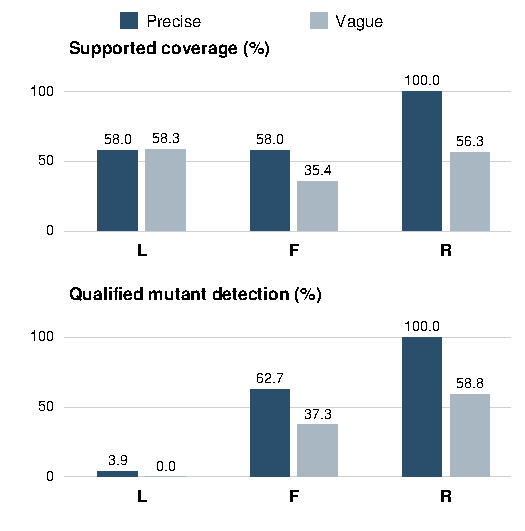
\includegraphics[width=\columnwidth]{api-rates.pdf}
\caption{API pilot rates. Supported coverage uses all supported candidate opportunities. Qualified detection uses all associated mutant opportunities. L, F, and R denote LLM, filtered, and rules. Fractions and counting units appear in Table~\ref{tab:api}.}
\label{fig:rates}
\Description{Two panels compare supported coverage and qualified mutant detection for the raw LLM, the filtered LLM, and deterministic rules under precise and vague requirements.}
\end{figure}

\subsection{RQ3: Qualified Fault Detection}
On precise API requirements, qualified detections increase from 2/51 to 32/51 after filtering, or from 3.9\% to 62.7\%. On vague requirements they increase from 0/51 to 19/51, or from 0\% to 37.3\%. The rule-only baseline has the highest observed rates, 17/17 on precise requirements and 10/17 on vague requirements.

These changes occur with unchanged action sequences and the same recorded service outcomes. Filtering improves qualification by removing unsupported checks or checks that fail on the original observation. Under the scoring rule, an unqualified suite contributes zero qualified kills even if some of its assertions can distinguish a mutant. Thus, changes in qualified kills combine suite validity and detection strength.

For example, on vague requirements the raw model has two suites passing the original service and three mutant detections if only original compatibility is required. Those suites contain unsupported assertions, so none of their detections qualifies under the full criterion. The filtered configuration has 12 nonempty passing suites, all supported, and detects 19 mutant opportunities. The increase reflects the definition and the resulting valid selections.

The observable-candidate denominator offers a second view. Four vague-variant mutants cannot be distinguished by any supported candidate in the fixed menu. Over the remaining 13 mutants, the filter obtains $19/39=48.7\%$ and rules obtain $10/13=76.9\%$. The raw all-mutant denominators retain the influence of requirement detail and candidate expressiveness. The restricted denominators show the selectors' performance within that expressiveness limit.

\subsection{Breakdown by Requirement and Seed}
Table~\ref{tab:byreq} decomposes the vague filtered row. Requirement 13 retains all six supported opportunities across the three seeds and detects six of nine mutant opportunities. Requirement 34 yields an empty filtered selection for each seed, giving zero of nine detections. These differences explain why an aggregate result can hide distinct failure mechanisms.

\begin{table}[t]
\caption{Vague filtered selections by requirement, summed over three seeds. Qualified counts nonempty supported suites that pass the original service.}
\label{tab:byreq}
\centering\small
\begin{tabular}{rrrr}
\toprule
ID & Supported & Qualified & Qualified kills\\
\midrule
2 & 2/15 & 2/3 & 2/9\\
3 & 2/6 & 2/3 & 4/6\\
4 & 2/3 & 2/3 & 4/9\\
6 & 5/15 & 3/3 & 3/9\\
13 & 6/6 & 3/3 & 6/9\\
34 & 0/3 & 0/3 & 0/9\\
\midrule
Total & 17/48 & 12/18 & 19/51\\
\bottomrule
\end{tabular}
\end{table}

Requirement 2 has 15 supported opportunities but retains only two. A low count can result from either the model omitting useful candidates or the rule selector failing to match supported wording. Requirement 6 retains five of 15 supported opportunities and qualifies for all three seeds, yet detects three of nine mutant opportunities. Qualification and detection therefore describe different aspects of the selected suite.

For seeds 11, 23, and 47, the vague filtered configuration retains five, seven, and five supported assertions. It qualifies for four, five, and three of the six requirements and detects six, eight, and five of 17 mutant opportunities respectively. Summing the supported selections gives 17. Summing the detection counts gives 19. Each seed uses the same six requirements and 17 mutant observations.

The small repeated sample supports descriptive counts. Requirements and their mutants form related observations, and seeds repeat the same tasks. Statistical inference about new projects would require a broader design with appropriate grouping and repeated execution.

\section{RQ4: A Larger Model and Frozen Rules}
\label{sec:followup}

\subsection{Paired Design}
We compared Qwen2.5-0.5B-Instruct and Qwen2.5-7B-Instruct in Q4\_K\_M format.\footnote{The official 7B model card and weights are at \url{https://huggingface.co/Qwen/Qwen2.5-7B-Instruct-GGUF}.} Both models used llama.cpp b5046, the same Vulkan runtime, a 2048-token context, and the original API prompts, grammar, temperature 0.3, top-$k$ 40, top-$p$ 0.95, and seeds 11, 23, and 47. We enabled prompt-prefix caching for both models after a CPU-only 7B trial exceeded the request timeout. The archived controlled-language pilot uses only the 0.5B model. Each follow-up model makes 36 FastAPI completions. Scoring reuses the same 23 recorded FastAPI responses and semantic labels from the diagnostic pilot.

We froze the rule implementation and held-out selection criteria in Git before screening TodoApp requirements from the same pinned RESTestBench revision. We screened 14 IDs in ascending order, selected the first eligible requirement for each distinct HTTP method and route, and found four eligible pairs under a cap of six. The pairs concern a rejected creation and successful retrieval, deletion, and update of a todo. We froze the two requirement variants per pair and their support labels before running inference. Gold labels come from one annotation set with recorded rationales. TodoApp contributes 24 completions per model and uses an eight-candidate status menu from the original rule vocabulary. We measure support and retention on TodoApp, with fault detection evaluated on the FastAPI records. The TodoApp status menu leaves body obligations and persistence outside the measured candidate space.

\subsection{Matched FastAPI Comparison}
Table~\ref{tab:api-model-size} reports the matched Vulkan comparison under the original support labels, alongside raw unsupported selections and unvetted original-compatible kills (mutant failures on suites that pass the reference service before checking requirement support). On vague requirements, scaling from 0.5B to 7B lowers the raw unsupported rate from $49/80$ (61.3\%) to $31/67$ (46.3\%) and raises raw supported coverage from $31/48$ to $36/48$. After intersection filtering, supported coverage moves from $18/48$ (58.1\% of raw supported choices retained) to $20/48$ (55.6\% retained), with zero unsupported selections under the original labels, while qualified detections move from $22/51$ to $21/51$. On precise text, filtered coverage moves from $50/81$ to $47/81$ and qualified detections from $36/51$ to $37/51$.

\begin{table*}[t]
\caption{Matched FastAPI model comparison under Vulkan (three seeds: 18 suites and 51 mutant opportunities per row). Compat.\ kills count mutant detections by nonempty suites passing the original service prior to support qualification; Qual.\ kills additionally require every selected assertion to belong to $G_r$.}
\label{tab:api-model-size}
\centering\small
\begin{tabular}{llrrrrrrr}
\toprule
 & & \multicolumn{4}{c}{Raw LLM ($L$)} & \multicolumn{3}{c}{Filtered Intersection ($F=L\cap R$)}\\
\cmidrule(lr){3-6}\cmidrule(lr){7-9}
Variant & Model & Supported & Unsupported & Orig.\ pass & Compat.\ / Qual.\ kills & Supported & Empty & Qual.\ kills\\
\midrule
Precise & 0.5B & 50/81 & 23/73 & 4/18 & 7/51 / \phantom{0}7/51 & 50/81 & 2/18 & 36/51\\
Precise & 7B   & 47/81 & 14/61 & 7/18 & 18/51 / 18/51 & 47/81 & 0/18 & 37/51\\
\midrule
Vague   & 0.5B & 31/48 & 49/80 & 1/18 & 2/51 / \phantom{0}2/51 & 18/48 & 5/18 & 22/51\\
Vague   & 7B   & 36/48 & 31/67 & 8/18 & 23/51 / \phantom{0}5/51 & 20/48 & 4/18 & 21/51\\
\bottomrule
\end{tabular}
\end{table*}

Crucially, on vague requirements the raw 7B model achieves $8/18$ original-passing suites and $23/51$ compatible mutant kills, up from $1/18$ and $2/51$ at 0.5B, yet $18$ of those $23$ detections come from six suites that assert unstated implementation conventions (such as exact \texttt{http\_200}, \texttt{http\_400}, or \texttt{can\_login} checks) and therefore fail support qualification ($5/51$ qualified kills). A benchmark that grades generated tests solely by reference compatibility and mutant kills would credit those $23/51$ detections, masking specification-oracle drift as model capability increases \cite{konstantinou2024,ding2026}.

The larger model also reduces seed-to-seed variance. Across seeds $(11,23,47)$, raw precise supported counts span $[12,24,14]$ at 0.5B (zero of six requirements unanimous across seeds) versus $[15,15,17]$ at 7B (two of six unanimous), with filtered precise kills stabilizing from $[11,16,9]$ to $[12,12,13]$. Meanwhile, the matched Vulkan 0.5B run reproduces the discrete selection mask of the archived CPU run on only $16/36$ FastAPI calls, whereas an exact CPU rerun with the archived settings matches $36/36$ FastAPI and $144/144$ controlled completions. Changing the execution backend and KV-cache prefix reuse under 4-bit quantization and non-zero temperature ($\tau=0.3$) shifts $55.6\%$ of individual 0.5B masks without altering the qualitative filtering effect, reinforcing methodological warnings on inference-stack sensitivity \cite{sallou2024}.

The aggregate shift from $22/51$ to $21/51$ vague qualified detections combines opposing requirement-level effects (Table~\ref{tab:api-scale-by-requirement}, traced to \href{https://github.com/lythean2508/Evaluating-LLM-Selected-Test-Oracles-for-Underspecified-Natural-Language-Requirements/blob/main/followup/results/api-vague-filtered-by-requirement.csv}{\texttt{api-vague-filtered-by-requirement.csv}}). At 7B, requirement~6 improves from $2/9$ to $5/9$ kills and requirement~34 recovers from $0/9$ (three empty suites at 0.5B) to $3/9$, whereas requirement~4 drops from $6/9$ to $2/9$ because 7B omits the broad \texttt{denied} check in seeds~11 and~23 in favor of exact status checks that the vague policy excludes.

\begin{table}[t]
\caption{Filtered results for vague FastAPI requirements across three seeds under Vulkan. Coverage divides supported selections by available supported candidates. Kills count qualified detections over mutant opportunities.}
\label{tab:api-scale-by-requirement}
\centering\small
\begin{tabular}{lrrrr}
\toprule
 & \multicolumn{2}{c}{Coverage} & \multicolumn{2}{c}{Kills}\\
ID & 0.5B & 7B & 0.5B & 7B\\
\midrule
2  & 2/15 & 1/15 & 2/9 & 1/9\\
3  & 3/6  & 3/6  & 6/6 & 6/6\\
4  & 3/3  & 1/3  & 6/9 & 2/9\\
6  & 4/15 & 8/15 & 2/9 & 5/9\\
13 & 6/6  & 4/6  & 6/9 & 4/9\\
34 & 0/3  & 3/3  & 0/9 & 3/9\\
\midrule
Total & 18/48 & 20/48 & 22/51 & 21/51\\
\bottomrule
\end{tabular}
\end{table}

\subsection{Held-out TodoApp Requirements}
Table~\ref{tab:heldout-status} reports status-oracle outcomes on the four held-out TodoApp pairs. On precise text, 7B raises raw supported coverage from $7/24$ to $13/24$, lowers raw unsupported selections from $42/49$ to $19/32$, and raises filtered coverage from $7/24$ to $10/24$ while cutting empty suites from $6/12$ to $2/12$. On vague text, 0.5B and 7B select $5/12$ and $3/12$ supported opportunities before filtering, but the frozen rules match zero status candidates on all four vague phrasings (e.g., \emph{``returns a validation error''}, \emph{``returns the correct todo''}, \emph{``removes it from the database''}, and \emph{``correctly changes its fields''}), forcing $12/12$ empty filtered suites for both models.

\begin{table}[t]
\caption{Held-out TodoApp status assertions (three seeds: 12 suites per row). Coverage uses available supported candidates. Unsupported uses all filtered selections. Empty uses all filtered suites. A dash marks zero selected assertions.}
\label{tab:heldout-status}
\centering\small
\setlength{\tabcolsep}{4pt}
\begin{tabular}{llrrrr}
\toprule
 & & \multicolumn{2}{c}{Coverage} & \multicolumn{2}{c}{Filtered}\\
Variant & Model & Raw & Filtered & Unsupported & Empty\\
\midrule
Precise & 0.5B & 7/24 & 7/24 & 2/9 & 6/12\\
Precise & 7B & 13/24 & 10/24 & 3/13 & 2/12\\
Vague & 0.5B & 5/12 & 0/12 & -- & 12/12\\
Vague & 7B & 3/12 & 0/12 & -- & 12/12\\
\bottomrule
\end{tabular}
\end{table}

In one deterministic pass on precise TodoApp text, the frozen rules cover $7/8$ supported candidates (missing \texttt{http\_200} on requirement~9 because \emph{``Verify response is 200 OK''} omits the keywords \texttt{status} and \texttt{HTTP}) and introduce one unsupported candidate. Specifically, requirement~6 specifies \texttt{200 OK} for \texttt{DELETE /todos/\{id\}} followed by \texttt{404 Not Found} on a subsequent verification \texttt{GET}. Because the document-level regex selector is step-agnostic, \texttt{404} triggers \texttt{denied}, yielding the mutually contradictory rule suite $\{\texttt{http\_200},\texttt{success},\texttt{denied}\}$ ($2\text{xx}\wedge 4\text{xx}$), which violates original-service compatibility and thus breaks the qualification precondition $Q(R,r)$ of Equation~\ref{eq:bound}. Moreover, both 0.5B (in two seeds) and 7B (in all three seeds, selecting $\{\texttt{http\_200},\texttt{denied}\}$) exhibit the same cross-step scope confusion, so correlated error across $L$ and $R$ preserves an unsatisfiable assertion pair in $2/9$ and $3/13$ filtered selections, respectively.

\subsection{Rule Ceiling and Sensitivity to Support Labels}
Table~\ref{tab:partition} decomposes supported FastAPI opportunities into four disjoint subsets across the archived CPU 0.5B run and the matched Vulkan pair. Under the original vague labels, the frozen rules impose an invariant ceiling of $27/48$ ($56.3\%$) supported opportunities across three seeds. Scaling from 0.5B to 7B under Vulkan shrinks model-missed rule matches ($R$ only) from $9$ to $7$ and joint omissions from $8$ to $5$, but simultaneously increases supported model choices vetoed by the lexical gate ($L$ only) from $13$ to $16$. Regardless of model capacity, intersection filtering cannot recover candidates in $G_r\setminus R(r)$. On vague TodoApp, $R(r)=\emptyset$ prior to label scoring, so the $12/12$ empty suites hold under every possible support annotation.

\begin{table}[t]
\caption{Disjoint partition of supported FastAPI candidate opportunities across three seeds under original labels ($G_r$). $L$ only counts supported model choices vetoed by rules; $R$ only counts rule matches omitted by the model; Ceiling is $|G_r\cap R|$.}
\label{tab:partition}
\centering\small
\setlength{\tabcolsep}{3.0pt}
\begin{tabular}{llrrrrrr}
\toprule
Variant & Run / Model & Both & $L$ only & $R$ only & Neither & Ceiling & $|G_r|$\\
\midrule
Precise & 0.5B (CPU) & 47 & 0 & 34 & 0 & 81 & 81\\
Precise & 0.5B (Vulkan) & 50 & 0 & 31 & 0 & 81 & 81\\
Precise & 7B (Vulkan) & 47 & 0 & 34 & 0 & 81 & 81\\
\midrule
Vague & 0.5B (CPU) & 17 & 11 & 10 & 10 & 27 & 48\\
Vague & 0.5B (Vulkan) & 18 & 13 & 9 & 8 & 27 & 48\\
Vague & 7B (Vulkan) & 20 & 16 & 7 & 5 & 27 & 48\\
\bottomrule
\end{tabular}
\end{table}

To test sensitivity to interpretive policy, we replayed the FastAPI suites across all $2^3=8$ combinations of three stricter annotation rules surfaced during an exploratory AI-assisted review: requiring explicit numeric wording for \texttt{http\_404} on vague not-found text (R3), requiring explicit response-body wording rather than state-update wording for \texttt{PUT} fields (four checks in R6), and requiring explicit token wording for the compound \texttt{can\_login} check (R34). Enabling a switch removes the affected check(s) from $G_r$ while keeping all saved selections and API observations fixed.

Under baseline policy \texttt{000}, filtered vague coverage favors 7B over 0.5B ($20/48$ vs.\ $18/48$). Activating the stricter \texttt{PUT}-field policy reverses this ranking across all four corresponding policies (e.g., $14/36$ vs.\ $16/36$ under \texttt{010}, and $14/33$ vs.\ $16/33$ with $6/20$ vs.\ $2/18$ unsupported selections under \texttt{111}), because 7B more frequently selects \texttt{same\_owner} on R6 where rules also match. Conversely, vague qualified detections remain lower at 7B across all eight policies ($21/51$ vs.\ $22/51$ without \texttt{PUT} restriction; $16/51$ vs.\ $20/51$ with it), and precise qualified detections flip from $37/51$ vs.\ $36/51$ to $28/51$ vs.\ $31/51$ whenever explicit token wording is required (\texttt{001}, \texttt{011}, \texttt{101}, \texttt{111}). Model-scaling conclusions on underspecified requirements are therefore policy-contingent, motivating blind multi-rater adjudication before claiming superiority.


\section{Worked Example: Access to Another User's Item}
RESTestBench requirement 4 concerns reading an item owned by another user. The vague variant asks the tester to verify that a second user cannot read that item and that access is denied. The precise variant specifies registration, authentication, item creation, the second user's access attempt, HTTP 400, and the JSON detail text \texttt{Not enough permissions}. These variants have different supported assertion sets in the pilot.

For the vague variant, the annotation set contains only \texttt{denied}, implemented as a 4xx status-class check. For the precise variant it additionally contains \texttt{http\_400} and \texttt{no\_permission}. This policy allows a direct demonstration of what increasing requirement detail makes observable to a supported oracle.

The fixed scenario creates two ordinary accounts, authenticates them, creates an item as the first account, and retrieves it as the second. The original observation returns HTTP 400 with the expected permission detail. One associated mutant retains HTTP 400 and changes the detail to \texttt{Item not found}. Table~\ref{tab:example} shows how the two checks behave on these responses.

\begin{table}[t]
\caption{Requirement 4 message-changing mutant. The detailed check detects the changed message under the precise requirement.}
\label{tab:example}
\centering\small
\begin{tabular}{@{}p{0.41\columnwidth} p{0.24\columnwidth} p{0.24\columnwidth}@{}}
\toprule
Observation or check & Original & Mutant\\
\midrule
HTTP status & 400 & 400\\
JSON detail & {\raggedright Not enough permissions\par} & {\raggedright Item not found\par}\\
Status is 4xx & Pass & Pass\\
{\raggedright Status is 400 and detail matches\par} & Pass & Fail\\
\bottomrule
\end{tabular}
\end{table}

The broad check continues to pass after the message change. The detailed check fails on the mutant because the precise requirement fixes that message. The mutant is outside the vague variant's supported observation capability in this menu. This example explains the difference between every associated mutant and every candidate-observable mutant in the detection denominator.

An exact code or detail can also be coincidentally correct on the original implementation while lacking textual support in the vague variant. Such a check is excluded by the qualification policy. Checking the code's current response alone would provide evidence of compatibility, while the requirement-support annotation records whether the test imposes a stated obligation.

The demonstration script reproduces this distinction with actual HTTP requests. It launches an isolated Docker Compose project, checks the original service, applies the benchmark mutation, restarts the backend, verifies the running source file against its local digest, and repeats the scenario. The project is then stopped and its temporary resources are removed. This single live example illustrates the mechanism underlying the saved evaluation.

\section{Discussion}
\subsection{What the Filter Achieves}
The pilots show that agreement filtering can remove unsupported choices made by a small model under a fixed candidate representation. In the API sample it also increases the number of nonempty suites that pass the original service. The detailed coverage counts show when this improvement comes with the loss of supported assertions. These observations support evaluating a filter along both selection support and fault detection.

The controlled and API tasks expose different retention patterns. In the finite grammar, the rule selector covers every determined probe and preserves all correct choices made by the abstention prompt. In the API sample, phrase-based rules cover only part of the supported vague menu and discard 11 correct raw selections. The latter case is more representative of the incompleteness expected from a small manually written phrase library.

\subsection{The Role of the Rule-Only Baseline}
The rule-only baseline achieves the highest detection rate in both API requirement variants. The intersection is bounded by the rule set and can lose an assertion that rules selected correctly when the model omits it. The observed data therefore favor rules alone for this particular sample and annotation policy. In this diagnostic design, the rule-only configuration provides an informative reference for the omissions introduced by the additional model-selection stage. The comparison identifies when agreement filtering improves the validity of selected suites and when its retention bottleneck reduces their detection capability.

Rules were written after reading the FastAPI samples. The controlled grammar was crafted to admit finite interpretation. These choices favor the rules in their development setting. Section~\ref{sec:followup} measures transfer of the exact API rules to another service.

\subsection{From Oracle Selection to Test Generation}
The experimental harness supplies action sequences, authentication setup, candidate checks, and response evaluators. A complete generation workflow also needs to construct these artifacts, maintain state, choose data, and produce executable code. Existing acceptance-test and REST workflows address portions of that wider problem \cite{ferreira2025,kogler2025restifai}. Our measurements isolate the final selection decision inside such a workflow.

An extended system could attach an evidence span to each assertion, distinguish assumptions from stated obligations, and request clarification for a missing code or boundary. Evaluating that design would require measures for evidence accuracy, reviewer effort, and the handling of empty selections. These are proposed extensions arising from the observed failure modes.

\subsection{Independent Annotation}
An independent annotation exercise should ask two human raters to label candidates using the visible requirement variant, fixed scenario, and a written interpretation policy. The FastAPI menu contains 44 candidates per variant, yielding 88 binary decisions per rater. Initial labeling should blind raters to model selections, rule matches, and mutant outcomes. Report the confusion matrix, raw agreement, and Cohen's kappa for the nominal labels before adjudication \cite{cohen1960}, then rescore all configurations under the adjudicated labels.

\section{Threats to Validity}
\subsection{Construct Validity}
Requirement support is operationalized by finite interpretations in the controlled task and a study-authored annotation set in the API task. Interpreting denial as a 4xx check is a policy choice. Broader domain conventions or a different interface contract could support a different set. The saved labels make this decision inspectable, and a label revision should trigger rescoring.

The candidate menus constrain what can be expressed and detected. A supported oracle outside the menu cannot contribute to coverage or mutant detection. Four vague-variant mutants remain indistinguishable under the available supported candidates. The secondary observable denominator makes this limitation explicit, while the primary denominator retains its practical effect.

Qualified kills combine support, nonemptiness, original pass, and mutant failure. A low value can arise through any of these components. Reporting all components avoids interpreting a change in qualification as a pure improvement in behavioral strength. Assertions such as a general success check and an exact status check can overlap semantically, so coverage counts reflect the supplied menu.

\subsection{Internal Validity}
The API labels and phrase rules were developed within the same small study. Separate files distinguish their roles, but their preparation is subject to shared judgment. The study includes one annotation set and lacks a measured inter-rater agreement estimate. A blind independent annotation exercise would strengthen the semantic evaluation.

The rules were informed by the sample text. This favors the deterministic baseline and can overstate filter reliability on future requirements. The finite grammar similarly favors the enumerating selector. Our results should be read together with these design facts.

Recorded API outcomes are reused for every selected suite. This controls state and execution variability across methods, while preventing the scoring stage from measuring flakiness or request-generation failures. A full replication should repeat service executions and check dependencies, timings, and database initialization.

\subsection{External and Conclusion Validity}
The model-size comparison uses two quantized models from one family. It covers English requirements and fixed candidate menus. FastAPI covers 17 distinct seeded faults and 51 scored opportunities per model configuration. TodoApp contributes one held-out service, four requirement pairs, and an assertion menu restricted to response status. Its labels were prepared by one annotator and training overlap was unaudited. The three seeds repeat the same tasks. Transfer to other projects, languages, model families, and assertion representations requires broader coverage.

Benchmark artifacts are publicly available. Model training overlap has not been independently audited. Work using post-cutoff oracle datasets illustrates one way to examine this issue \cite{molinelli2025}. Fixed inputs and constrained decoding also change the difficulty relative to free-form test generation.

A held-out fault-detection study should execute the fixed TodoApp scenarios against the original service and requirement-associated mutants, using the property-based and requirements-based mutation designs of Bartocci et al. and RESTestBench \cite{bartocci2023,kogler2026bench}. The same observations can be scored for all selectors under the qualification rule in Section~\ref{sec:measures}. Reporting associated and candidate-observable mutant counts would expose limits imposed by the status menu.

The expanded analyses are descriptive. Counts repeated across seeds are dependent on the same requirements and observations. We report their exact denominators and avoid treating 51 evaluations as 51 independent software faults. Mutation operators approximate selected error mechanisms, so rates on these mutants provide scoped evidence about test behavior \cite{papadakis2019,bartocci2023}.

\section{Reproducibility}
The supplementary replication materials contain the controlled threshold data, API requirement extracts, model responses, API observations, and scorers. The archive verifier reproduces the original pilots. The \texttt{followup/} directory contains the protocol freeze, held-out source and labels, raw completions, model checksums, and a separate API replay command. Appendix~\ref{app:replay} gives the archived pilot filenames and command.

There are three reproduction levels. Rescoring reads the saved model responses and API outcomes. Regeneration executes new model calls using the frozen prompts, model, grammar, and sampler configuration. Live execution reruns API scenarios against the original and mutated services. Rescoring verifies the transformation from raw records to tables. Regeneration and repeated execution assess repeatability under a specified runtime.

The benchmark repository checkout and the FastAPI Docker image remain dependencies of the live demonstration. The archive-based scoring path uses standard Python facilities. Runtime paths should be configured for the current machine, and model weights and Docker dependencies should be available before a live presentation. Appendix~\ref{app:replay} gives the short scoring procedure and its expected output.

\section{Conclusion}
We studied assertion selection for test cases derived from complete and underspecified natural-language requirements. A small Qwen model, deterministic text rules, and their intersection were evaluated with fixed probes and fixed API scenarios. Filtering removed the observed unsupported selections in both pilots. On vague API requirements it reduced supported coverage from 28/48 to 17/48 while increasing qualified detections from 0/51 to 19/51. Rules alone achieved the highest observed detection rates under the sampled texts and annotation policy.

Under matched inference settings, 7B retains two more supported selections on vague FastAPI requirements, while qualified detections decrease by one. Both models return empty filtered suites for all vague TodoApp evaluations because the frozen rules match none of the supported status checks. Model scaling helps some selections and leaves the rule-coverage limit in place. Broader service coverage and independent support annotation would test the stability of this result.

\section*{Data Availability Statement}
The \href{https://github.com/lythean2508/Evaluating-LLM-Selected-Test-Oracles-for-Underspecified-Natural-Language-Requirements}{public replication repository} archives the diagnostic pilots in release \texttt{v1.0.0}. The \texttt{followup/} directory documents the paired API study, provides its completion logs, and gives separate commands for rescoring and regeneration.

\appendix
\section{Replaying the Stored Evidence}
\label{app:replay}
The supplementary package contains the following two data archives and verification script.
\begin{quote}\small\ttfamily
replication-controlled-pilot.zip\\
replication-restestbench-pilot.zip\\
verify\_paper\_results.py
\end{quote}
Keep these three files in the same folder. Use Python 3.12 or later and open a terminal in that folder. Run
\begin{quote}\small\ttfamily
python verify\_paper\_results.py score
\end{quote}
The first displayed pilot should contain 58/126, 0/126, 29/126, and 42/42. The API table should contain all six rows of Table~\ref{tab:api}. The final PASS message confirms that rescoring agrees with the frozen summaries. The stored raw files remain available for inspection in the printed replay location.

\noindent\begin{minipage}{\columnwidth}
For an arithmetic spot check, sum the vague filtered row of the per-requirement table. Supported retention is $(2+2+2+5+6+0)/48=17/48$. Qualified detections are $(2+4+4+3+6+0)/51=19/51$. The alternative seed sum is $(6+8+5)/51=19/51$. These are two decompositions of the same saved evaluations.
\end{minipage}\par

The live demonstration additionally needs a Python environment with the API-script dependencies, Docker Desktop with a running Linux Engine, the existing benchmark checkout, and the frozen backend and PostgreSQL images. Its mode is \texttt{live}. The original response should be HTTP 400 with permission detail and the mutant response HTTP 400 with item-not-found detail. The detailed assertion's failure on the mutant is the expected detection event.

\section{Interpretation Audit}
The controlled denominator 126 counts 42 probe positions over three seeds. The vague API denominator 48 counts 16 supported menu candidates over three seeds. The precise denominator 81 counts 27 supported candidates over three seeds. The detection denominator 51 counts 17 mutants over three seeds. These denominators represent different quantities and should be retained when presenting percentage results.

For the vague filtered method, zero unsupported assertions means zero among 17 retained selections. Six of the 18 suites are empty. For precise requirements, keeping all 47 supported raw selections means preserving those already selected, with 81 supported opportunities available overall. These distinctions make it possible to explain the paper's results using the raw records and the evaluation policy.

\balance
\begin{thebibliography}{99}
\bibitem{barr2015} Earl T. Barr, Mark Harman, Phil McMinn et al. 2015. The Oracle Problem in Software Testing: A Survey. \emph{IEEE Transactions on Software Engineering 41(5), 507-525}. \url{https://doi.org/10.1109/TSE.2014.2372785}.

\bibitem{yang2025} Zhenzhen Yang, Rubing Huang, Chenhui Cui et al. 2026. Requirements-Based Test Generation: A Comprehensive Survey. \emph{ACM TOSEM, accepted manuscript}. \url{https://doi.org/10.1145/3771727}.

\bibitem{wang2024survey} Junjie Wang, Yuchao Huang, Chunyang Chen et al. 2024. Software Testing with Large Language Models: Survey, Landscape, and Vision. \emph{IEEE Transactions on Software Engineering 50(4), 911-936}. \url{https://doi.org/10.1109/TSE.2024.3368208}.

\bibitem{folorunsho2026} Orimoloye Folorunsho, Hassan Reza. 2026. AI-Driven Test Case Generation from Natural Language Requirements: A Survey of Techniques and Research Gaps. \emph{Preprint}. \url{https://arxiv.org/abs/2606.06563}.

\bibitem{wang2022umtg} Chunhui Wang, Fabrizio Pastore, Arda Goknil et al. 2022. Automatic Generation of Acceptance Test Cases from Use Case Specifications: An NLP-Based Approach. \emph{IEEE Transactions on Software Engineering 48(2), 585-616}. \url{https://doi.org/10.1109/TSE.2020.2998503}.

\bibitem{fischbach2023} Jannik Fischbach, Julian Frattini, Andreas Vogelsang et al. 2023. Automatic Creation of Acceptance Tests by Extracting Conditionals from Requirements: NLP Approach and Case Study. \emph{Journal of Systems and Software 197, 111549}. \url{https://doi.org/10.1016/j.jss.2022.111549}.

\bibitem{arora2024} Chetan Arora, Tomas Herda, Verena Homm. 2024. Generating Test Scenarios from NL Requirements using Retrieval-Augmented LLMs: An Industrial Study. \emph{IEEE International Requirements Engineering Conference}. \url{https://doi.org/10.1109/RE59067.2024.00031}.

\bibitem{ferreira2025} Margarida Ferreira, Luis Viegas, Joao Pascoal Faria et al. 2025. Acceptance Test Generation with Large Language Models: An Industrial Case Study. \emph{IEEE/ACM International Conference on Automation of Software Test}. \url{https://doi.org/10.1109/AST66626.2025.00007}.

\bibitem{masuda2025} Satoshi Masuda, Satoshi Kouzawa, Kyousuke Sezai et al. 2025. Generating High-Level Test Cases from Requirements using LLM: An Industry Study. \emph{Preprint}. \url{https://arxiv.org/abs/2510.03641}.

\bibitem{moradi2026} Milad Moradi, Ke Yan, David Colwell et al. 2026. An empirical study of LoRA-based fine-tuning of large language models for automated test case generation. \emph{Preprint}. \url{https://arxiv.org/abs/2604.06946}.

\bibitem{xue2026} Zhiyi Xue, Xiaohong Chen, Min Zhang. 2026. Explicating Tacit Regulatory Knowledge from LLMs to Auto-Formalize Requirements for Compliance Test Case Generation. \emph{Preprint}. \url{https://arxiv.org/abs/2601.09762}.

\bibitem{endres2024} Madeline Endres, Sarah Fakhoury, Saikat Chakraborty et al. 2024. Can Large Language Models Transform Natural Language Intent into Formal Method Postconditions?. \emph{Proceedings of the ACM on Software Engineering}. \url{https://doi.org/10.1145/3660791}.

\bibitem{dinella2022} Elizabeth Dinella, Gabriel Ryan, Todd Mytkowicz et al. 2022. TOGA: A Neural Method for Test Oracle Generation. \emph{International Conference on Software Engineering}. \url{https://arxiv.org/abs/2109.09262}.

\bibitem{hossain2023} Soneya Binta Hossain, Antonio Filieri, Matthew B. Dwyer et al. 2023. Neural-Based Test Oracle Generation: A Large-scale Evaluation and Lessons Learned. \emph{ACM Joint European Software Engineering Conference and Symposium on the Foundations of Software Engineering}. \url{https://doi.org/10.1145/3611643.3616265}.

\bibitem{konstantinou2024} Michael Konstantinou, Renzo Degiovanni, Mike Papadakis. 2024. Do LLMs generate test oracles that capture the actual or the expected program behaviour?. \emph{Preprint}. \url{https://arxiv.org/abs/2410.21136}.

\bibitem{molinelli2025} Davide Molinelli, Luca Di Grazia, Alberto Martin-Lopez et al. 2025. Do LLMs Generate Useful Test Oracles? An Empirical Study with an Unbiased Dataset. \emph{IEEE/ACM International Conference on Automated Software Engineering, 278-290}. \url{https://homes.cs.washington.edu/~mernst/pubs/neurosymbolic-oracles-ase2025-abstract.html}.

\bibitem{ouedraogo2024} Wendkuuni C. Ouedraogo, Kader Kabore, Yewei Song et al. 2024. LLMs and Prompting for Unit Test Generation: A Large-Scale Evaluation. \emph{IEEE/ACM International Conference on Automated Software Engineering, 2464-2465}. \url{https://doi.org/10.1145/3691620.3695330}.

\bibitem{kogler2026bench} Leon Kogler, Stefan Hangler, Maximilian Ehrhart et al. 2026. RESTestBench: A Benchmark for Evaluating the Effectiveness of LLM-Generated REST API Test Cases from NL Requirements. \emph{EASE 2026 author manuscript}. \url{https://arxiv.org/abs/2604.25862}.

\bibitem{ma2026} Tiancheng Ma, Nasir U. Eisty. 2026. From Business Requirements to Test Assertions: Evaluating LLM-Generated Oracles on Real Bugs. \emph{Preprint}. \url{https://arxiv.org/abs/2607.10277}.

\bibitem{shi2026} Yunjiao Shi, Rui Song. 2026. ReqTestAgent: execution-grounded language-model agents for acceptance testing under requirement ambiguity. \emph{Frontiers in Artificial Intelligence 9, 1960601}. \url{https://doi.org/10.3389/frai.2026.1960601}.

\bibitem{qi2026} Binhang Qi, Yiming Liu, Yun Lin et al. 2026. Benchmarking LLM Agents for Behaviorally Adequate Test Generation from Software Requirements. \emph{Preprint}. \url{https://arxiv.org/abs/2610.36584}.

\bibitem{kogler2025restifai} Leon Kogler, Maximilian Ehrhart, Benedikt Dornauer et al. 2025. RESTifAI: LLM-Based Workflow for Reusable REST API Testing. \emph{accepted ICSE 2026 demonstration}. \url{https://arxiv.org/abs/2512.08706}.

\bibitem{golmohammadi2024} Amid Golmohammadi, Man Zhang, Andrea Arcuri. 2024. Testing RESTful APIs: A Survey. \emph{ACM Transactions on Software Engineering and Methodology 33(1)}. \url{https://doi.org/10.1145/3617175}.

\bibitem{martinlopez2021} Alberto Martin-Lopez, Sergio Segura, Antonio Ruiz-Cortes. 2021. RESTest: Automated Black-Box Testing of RESTful Web APIs. \emph{ACM International Symposium on Software Testing and Analysis}. \url{https://personal.us.es/amarlop/wp-content/uploads/2021/06/RESTest-Automated-Black-Box-Testing-of-RESTful-Web-APIs.pdf}.

\bibitem{bartocci2023} Ezio Bartocci, Leonardo Mariani, Dejan Nickovic et al. 2023. Property-Based Mutation Testing. \emph{IEEE International Conference on Software Testing, Verification and Validation, 222-233}. \url{https://doi.org/10.1109/ICST57152.2023.00029}.

\bibitem{papadakis2019} Mike Papadakis, Marinos Kintis, Jie Zhang et al. 2019. Mutation Testing Advances: An Analysis and Survey. \emph{Advances in Computers 112, 275-378}. \url{https://doi.org/10.1016/bs.adcom.2018.03.015}.

\bibitem{cunha2026} Alcino Cunha, Nuno Macedo. 2026. Validating Formal Specifications with LLM-generated Test Cases. \emph{Preprint}. \url{https://arxiv.org/abs/2510.23350}.

\bibitem{qwen2024} Qwen Team. 2024. Qwen2.5-0.5B-Instruct-GGUF. \emph{Official model card}. \url{https://huggingface.co/Qwen/Qwen2.5-0.5B-Instruct-GGUF}.

\bibitem{llamacpp} llama.cpp contributors. 2025. llama.cpp, release b5046. \emph{Software release}. \url{https://github.com/ggml-org/llama.cpp/releases/tag/b5046}.

\bibitem{fastapi} FastAPI contributors. 2026. Full Stack FastAPI Template. \emph{Source repository, accessed 19 November 2026}. \url{https://github.com/fastapi/full-stack-fastapi-template}.

\bibitem{openapi} OpenAPI Initiative. 2021. OpenAPI Specification, version 3.1.0. \emph{Interface specification}. \url{https://spec.openapis.org/oas/v3.1.0}.

\bibitem{restestrepo} RESTestBench authors. 2026. RESTestBench replication repository. \emph{Experiment checkout at commit 4decc1e36ea3dd41b64ce3e3ac6a85bc72df36ae}. \url{https://github.com/casablancahotelsoftware/RESTestBench}.

\bibitem{rbtgdata} SLR-on-RBTG authors. 2025. SLR-on-RBTG: collection of 267 primary studies. \emph{Survey companion repository}. \url{https://github.com/aimeenorwind/SLR-on-RBTG}.

\bibitem{cohen1960} Jacob Cohen. 1960. A Coefficient of Agreement for Nominal Scales. \emph{Educational and Psychological Measurement 20(1), 37--46}. \url{https://doi.org/10.1177/001316446002000104}.
\end{thebibliography}
\end{document}
